% !TEX program = pdflatex

\documentclass[a4paper,11pt,twoside]{report}
% THIS FILE SHOULD BE COMPILED BY pdfLaTeX

% ----------------------   PREAMBLE PART ------------------------------

% ------------------------ ENCODING & LANGUAGES ----------------------

\usepackage[utf8]{inputenc}
%\usepackage[MeX]{polski} % Not needed unless You have a name with polish symbols or sth
\usepackage[T1]{fontenc}
\usepackage[english, polish]{babel}


\usepackage{amsmath, amsfonts, amsthm, latexsym} % MOSTLY MATHEMATICAL SYMBOLS

\usepackage[final]{pdfpages} % INPUTING TITLE PDF PAGE - GENERATE IT FIRST!
%\usepackage[backend=bibtex, style=verbose-trad2]{biblatex}


\usepackage{commath} % various commands which can make writing math expressions easier --- documentation available at: https://ctan.gust.org.pl/tex-archive/macros/latex/contrib/commath/commath.pdf

\usepackage[hidelinks]{hyperref} % for hyperlinks, for example, urls, references to equations, entries in a bibliography --- hidelinks option removes rectangles around hiperlinks
\hypersetup{
    colorlinks=true,
    linkcolor=blue,
    filecolor=magenta,      
    urlcolor=cyan,
    pdftitle={Overleaf Example},
    pdfpagemode=FullScreen,
}
\usepackage{setspace}


% ---------------- MARGINS, INDENTATION, LINESPREAD ------------------

\usepackage[inner=20mm, outer=20mm, bindingoffset=10mm, top=25mm, bottom=25mm]{geometry} % MARGINS


\linespread{1.5}
\allowdisplaybreaks         % ALLOWS BREAKING PAGE IN MATH MODE

\usepackage{indentfirst}    % IT MAKES THE FIRST PARAGRAPH INDENTED; NOT NEEDED
\setlength{\parindent}{5mm} % WIDTH OF AN INDENTATION


%---------------- RUNNING HEAD - CHAPTER NAMES, PAGE NUMBERS ETC. -------------------

\usepackage{fancyhdr}
\pagestyle{fancy}
\fancyhf{}
% PAGINATION: LEFT ALIGNMENT ON EVEN PAGES, RIGHT ALIGNMENT ON ODD PAGES 
\fancyfoot[LE,RO]{\thepage} 
% RIGHT HEADER: zawartość \rightmark do lewego, wewnętrznego (marginesu) 
\fancyhead[LO]{\sc \nouppercase{\rightmark}}
% lewa pagina: zawartość \leftmark do prawego, wewnętrznego (marginesu) 
\fancyhead[RE]{\sc \leftmark}

\renewcommand{\chaptermark}[1]{\markboth{\thechapter.\ #1}{}}

% HEAD RULE - IT'S A LINE WHICH SEPARATES HEADER AND FOOTER FROM CONTENT
\renewcommand{\headrulewidth}{0 pt} % 0 MEANS NO RULE, 0.5 MEANS FINE RULE, THE BIGGER VALUE THE THICKER RULE


\fancypagestyle{plain}{
  \fancyhf{}
  \fancyfoot[LE,RO]{\thepage}
  
  \renewcommand{\headrulewidth}{0pt}
  \renewcommand{\footrulewidth}{0.0pt}
}

% SWOT 
\usepackage{xcolor}
\definecolor{swotS}{RGB}{226,237,143}
\definecolor{swotW}{RGB}{247,193,139}
\definecolor{swotO}{RGB}{173,208,187}
\definecolor{swotT}{RGB}{192,165,184}
\usepackage[raster]{tcolorbox}



% --------------------------- CHAPTER HEADERS ---------------------

\usepackage{titlesec}
\titleformat{\chapter}
  {\normalfont\Large \bfseries}
  {\thechapter.}{1ex}{\Large}

\titleformat{\section}
  {\normalfont\large\bfseries}
  {\thesection.}{1ex}{}
\titlespacing{\section}{0pt}{30pt}{20pt} 

    
\titleformat{\subsection}
  {\normalfont \bfseries}
  {\thesubsection.}{1ex}{}


% ----------------------- TABLE OF CONTENTS SETUP ---------------------------

\def\cleardoublepage{\clearpage\if@twoside
\ifodd\c@page\else\hbox{}\thispagestyle{empty}\newpage
\if@twocolumn\hbox{}\newpage\fi\fi\fi}


% THIS MAKES DOTS IN TOC FOR CHAPTERS
\usepackage{etoolbox}
\makeatletter
\patchcmd{\l@chapter}
  {\hfil}
  {\leaders\hbox{\normalfont$\m@th\mkern \@dotsep mu\hbox{.}\mkern \@dotsep mu$}\hfill}
  {}{}
\makeatother

\usepackage{titletoc}
\makeatletter
\titlecontents{chapter}% <section-type>
  [0pt]% <left>
  {}% <above-code>
  {\bfseries \thecontentslabel.\quad}% <numbered-entry-format>
  {\bfseries}% <numberless-entry-format>
  {\bfseries\leaders\hbox{\normalfont$\m@th\mkern \@dotsep mu\hbox{.}\mkern \@dotsep mu$}\hfill\contentspage}% <filler-page-format>

\titlecontents{section}
  [1em]
  {}
  {\thecontentslabel.\quad}
  {}
  {\leaders\hbox{\normalfont$\m@th\mkern \@dotsep mu\hbox{.}\mkern \@dotsep mu$}\hfill\contentspage}

\titlecontents{subsection}
  [2em]
  {}
  {\thecontentslabel.\quad}
  {}
  {\leaders\hbox{\normalfont$\m@th\mkern \@dotsep mu\hbox{.}\mkern \@dotsep mu$}\hfill\contentspage}
\makeatother



% ---------------------- TABLES AD FIGURES NUMBERING ----------------------

\renewcommand*{\thetable}{\arabic{chapter}.\arabic{table}}
\renewcommand*{\thefigure}{\arabic{chapter}.\arabic{figure}}


% ------------- DEFINING ENVIRONMENTS FOR THEOREMS, DEFINITIONS ETC. ---------------

\makeatletter
\newtheoremstyle{definition}
{3ex}%                           % Space above
{3ex}%                           % Space below
{\upshape}%                      % Body font
{}%                              % Indent amount
{\bfseries}%                     % Theorem head font
{.}%                             % Punctuation after theorem head
{.5em}%                          % Space after theorem head, ' ', or \newline
{\thmname{#1}\thmnumber{ #2}\thmnote{ (#3)}}
\makeatother

\theoremstyle{definition}
\newtheorem{theorem}{Theorem}[chapter]
\newtheorem{lemma}[theorem]{Lemma}
\newtheorem{example}[theorem]{Example}
\newtheorem{proposition}[theorem]{Proposition}
\newtheorem{corollary}[theorem]{Corollary}
\newtheorem{definition}[theorem]{Definition}
\newtheorem{remark}[theorem]{Remark}

% --------------------- END OF PREAMBLE PART (MOSTLY) --------------------------





% -------------------------- USER SETTINGS ---------------------------

\renewcommand{\title}{Platform for hybrid learning}
\newcommand{\type}{Engineer} % Master OR Engineer
\newcommand{\supervisor}{DEng Janusz Oleniacz} % TITLE AND NAME OF THE SUPERVISOR



\begin{document}
\sloppy
\selectlanguage{english}


\includepdf[pages=-]{titlepage} % THIS INPUTS THE TITLE PAGE

\null\thispagestyle{empty}\newpage

% ------------------ PAGE WITH SIGNATURES --------------------------------

%\thispagestyle{empty}\newpage
%\null
%
%\vfill
%
%\begin{center}
%\begin{tabular}[t]{ccc}
%............................................. & \hspace*{100pt} & .............................................\\
%supervisor's signature & \hspace*{100pt} & author's signature
%\end{tabular}
%\end{center}
%


% ---------------------------- ABSTRACTS -----------------------------

{  \fontsize{12}{14} \selectfont
\begin{abstract} 
	\begin{center}
		\title  
	\end{center}
The platform for hybrid learning intends to demonstrate, how the design of educational software could be done using a non-object-oriented approach alongside applying principles of cloud computing.
As students, during the pandemic of 2020-2021, we have seen how the educational system was struggling to handle such a change. Meanwhile, we have also discovered the advantages of studying online - it gave us a great level of flexibility and the possibility to re-access materials (in particular). Keeping in mind, that teachers would also benefit from the re-design of the current approach to knowledge transfer, we decided to try and implement a platform, that covers the interests of both groups. 
We did that using Rust programming language for our backend system, F\# programming language for the frontend (transpiled to JavaScript), and Azure as a main hosting solution. This paper addresses the obstacles to implementing such a platform and how it differs from already existing solutions. We used our professional knowledge as acting software engineers and students to identify and solve arising issues. 
It is worth adding, that we do not focus on the software development pipeline here, as it would differ vastly from the real-world development team. Nevertheless, we address usability, extendability, supportability, and other important software traits, since they are crucial to the success of the design itself. \\

\noindent \textbf{Keywords:} hydrid learning, massive open online courses, functional programming, cloud computing, education
\end{abstract}
}

\null\thispagestyle{empty}\newpage


% {\selectlanguage{polish} \fontsize{12}{14}\selectfont
% \begin{abstract}

% \begin{center}
% \tytul
% \end{center}

% Lorem ipsum dolor sit amet, consetetur sadipscing elitr, sed diam nonumyeirmod tempor invidunt ut labore et dolore magna aliquyam erat, sed diamvoluptua. At vero eos et accusam et justo duo dolores et ea rebum. Stet clita kasd gubergren, no sea takimata sanctus est Lorem ipsum dolor sit amet.

% Lorem ipsum dolor sit amet, consetetur sadipscing elitr, sed diam nonumyeirmod tempor invidunt ut labore et dolore magna aliquyam erat, sed diamvoluptua. At vero eos et accusam et justo duo dolores et ea rebum. Stet clita kasd gubergren, no sea takimata sanctus est Lorem ipsum dolor sit amet.\\

% \noindent \textbf{Słowa kluczowe:} slowo1, slowo2, ...
% \end{abstract}
% }


%% --------------------------- DECLARATIONS ------------------------------------
%
%%
%%	IT IS NECESSARY OT ATTACH FILLED-OUT AUTORSHIP DEECLRATION. SCAN (IN PDF FORMAT) NEEDS TO BE PLACED IN scans FOLDER AND IT SHOULD BE CALLED, FOR EXAMPLE, DECLARATION_OF_AUTORSHIP.PDF. IF THE FILENAME OR FILEPATH IS DIFFERENT, THE FILEPATH IN THE NEXT COMMAND HAS TO BE ADJUSTED ACCORDINGLY.
%%
%%	command attacging the declarations of autorship
%%
%\includepdf[pages=-]{scans/declaration-of-autorship}
%\null\thispagestyle{empty}\newpage
%
%% optional declaration
%%
%%	command attaching the declaataration on granting a license
%%
%\includepdf[pages=-]{scans/declaration-on-granting-a-license}
%%
%%	.tex corresponding to the above PDF files are present in the 3. declarations folder 
%
\chapter*{History of changes}
\begin{tabular}{ |p{3cm}|p{3cm}|p{7cm}|  }
 	\hline
 	\multicolumn{3}{|c|}{Table of changes} \\
 	\hline
 	Author & Date & Change\\
 	\hline
 	Kiryl Volkau   & 20.10.2021    & add: Abstract, Introduction \\
	Kiryl Volkau   & 20.10.2021    & add: Functional requirements \\
 	Illia Manzhela &  20.10.2021  & add: Non-functional requirements \\
 	Illia Manzhela &  20.10.2021  & add: SWOT analysis, schedule \\
 	\hline
\end{tabular}
% ------------------- TABLE OF CONTENTS ---------------------
% \selectlanguage{english} - for English
\pagenumbering{gobble}
\tableofcontents
\thispagestyle{empty}
\newpage % IF YOU HAVE EVEN QUANTITY OD PAGES OF TOC, THEN REMOVE IT OR ADD \null\newpage FOR DOUBLE BLANK PAGE BEFORE INTRODUCTION


% -------------------- THE BODY OF THE THESIS --------------------------------

\null\thispagestyle{empty}\newpage
\pagestyle{fancy}
\pagenumbering{arabic}
\setcounter{page}{11}

\chapter*{Vocabulary}
\markboth{}{Vocabulary}
\addcontentsline{toc}{chapter}{Vocabulary}


\begin{enumerate}
\item \textbf{Hybrid learning} - educational process, organised to be conducted both on-line and on-site, providing students and teachers with more flexibility and instant access to the educational materials.
\item \textbf{Massive Open Online Courses (MOOC)} platform - platform with educational content including videos, text content, discussion forums.
\item \textbf{Application Programming Interface (API)} - set of definitions for building and integrating application software.
\item \textbf{Infrastracture as a Service (IaaS)} - pay-as-you-go service where a third party provides you with infrastructure services, like storage and virtualization, as you need them, via a cloud, through the internet. \href{https://www.redhat.com/en/topics/cloud-computing/iaas-vs-paas-vs-saas}{https://www.redhat.com/en/topics/cloud-computing/iaas-vs-paas-vs-saas}
\item \textbf{Platform as a Service (PaaS)} - on-premise infrastructure management where a provider hosts the hardware and software on its own infrastructure and delivers this platform to the user as an integrated solution, solution stack, or service through an internet connection. \href{https://www.redhat.com/en/topics/cloud-computing/iaas-vs-paas-vs-saas}{https://www.redhat.com/en/topics/cloud-computing/iaas-vs-paas-vs-saas}
\end{enumerate}


\chapter*{Introduction}
\markboth{}{Introduction}
\addcontentsline{toc}{chapter}{Introduction}
Since the beginning of the COVID-19 pandemic, many academic institutions (including Warsaw University of Technologies) were forced to provide solutions for the transfer between on-site and on-line education formats. Moreover, today's educational systems get more and more criticism worldwide due to being too generic and inflexible \cite{onvsoff1}. Meanwhile, the popularity of platforms like Coursera (\href{https://www.coursera.org}{https://www.coursera.org}), Udemy (\href{https://www.udemy.com}{https://www.udemy.com}), Udacity (\href{https://www.udacity.com}{https://www.udacity.com}), etc. has been growing over the years. \\
\begin{figure}[hp]
\centering
    \begin{center}
        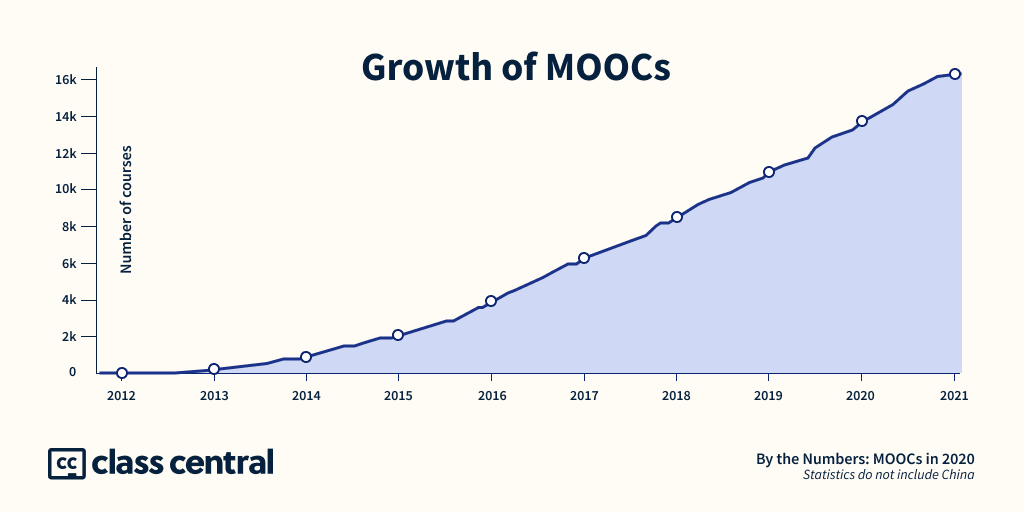
\includegraphics[scale=.4]{img/growth-2020.png}
          \caption{Growth of MOOC's platforms   \href{https://www.classcentral.com/report/mooc-stats-2020/}{https://www.classcentral.com/report/mooc-stats-2020/}\cite{growth}}
    \end{center}
\end{figure} \\
At the same time, it has also been shown that the main problem with MOOCs is that students are far more likely to drop the course without completing it \cite{dropout}. \\
As the authors of this thesis believe, the solution should lie somewhere in between. Education is not our area of expertise, so we ask readers to not treat us as the authority on the topic. Nevertheless, we do believe that there will be a shift toward more flexible education, as the continuity of life grows \cite{expectancy} alongside the pace of living \cite{pace}. So, in this paper, we aimed at providing one of possible solutions to the operational side of the matter: platform. Although, as has been mentioned by the experts \cite{harvard1}, the principles of student involvement in the subject remain the same, the strategy of implementing those principles should adapt and evolve. This is why, not being completely sure about the approaches taken by future generations of researchers, we design our platform with adaptivity and evolvability in mind. \\ 
We have decided to implement our platform using a less popular technological stack: Rust \cite{rust} for the backend and F\# \cite{fsharp} for the frontend (compiled to JavaScript using Fable \cite{fable}). Those are non-object-oriented languages greatly influenced by the functional programming paradigm. We go a little bit deeper into the topic in the following chapters, however, at the moment it is worth noticing the main strengths of the selected languages: 
\begin{enumerate}
	\item Algebraic data types - especially "sum", also known as "OR" type (discriminated union) - which allow us to express domain more exhaustively.
	\item Immutability dy default - most of the software operations could be represented as a pipeline of data transformation, and without some complex state management underneath (which is object-oriented approach is famous for) it becomes easier to decouple and modularize application. Decoupling and modularization are two approaches, with which we can empower the evolvability and adaptivity of our platform.
	\item Absence of null-value (in general), also known as a billion dollar mistake \cite{null}.
\end{enumerate}
The hosting is done on Azure \href{https://azure.microsoft.com/}{https://azure.microsoft.com/} due to its wide range of services and more clear billing, alongside some free student trials. \\ 
As for the potential competitors - there are multiple platforms with overlapping functionality / much more vast functionality (e.g. Moodle) already offered, than the one that we can deliver for a diploma thesis. Still, we do consider this project a solid basis for a future development - that's why it's code left open-source and we give specific recommendations and thoughts on extension of the existing codebase and functionality. However, we have not seen anything similar already developed or described somewhere as plans (it's worth noticing that the same functionality could be achieved using the set of multiple tools, but it just would be far less convenient).
\chapter*{Responsibilities and Schedule}
\markboth{}{Responsibilities and Schedule}
\addcontentsline{toc}{chapter}{Responsibilities and Schedule}
\begin{center}
\begin{tabular}{ |c|c| } 
 \hline
 Full Name & Responsibility \\ 
 \hline
 Kiryl Volkau & Frontend (Elm) \& DevOps (Azure) \\ 
 Illia Manzhella & Backend (Rust) \& DevOps (GitHub Actions) \\ 
 \hline
\end{tabular}
\begin{figure}[h]
    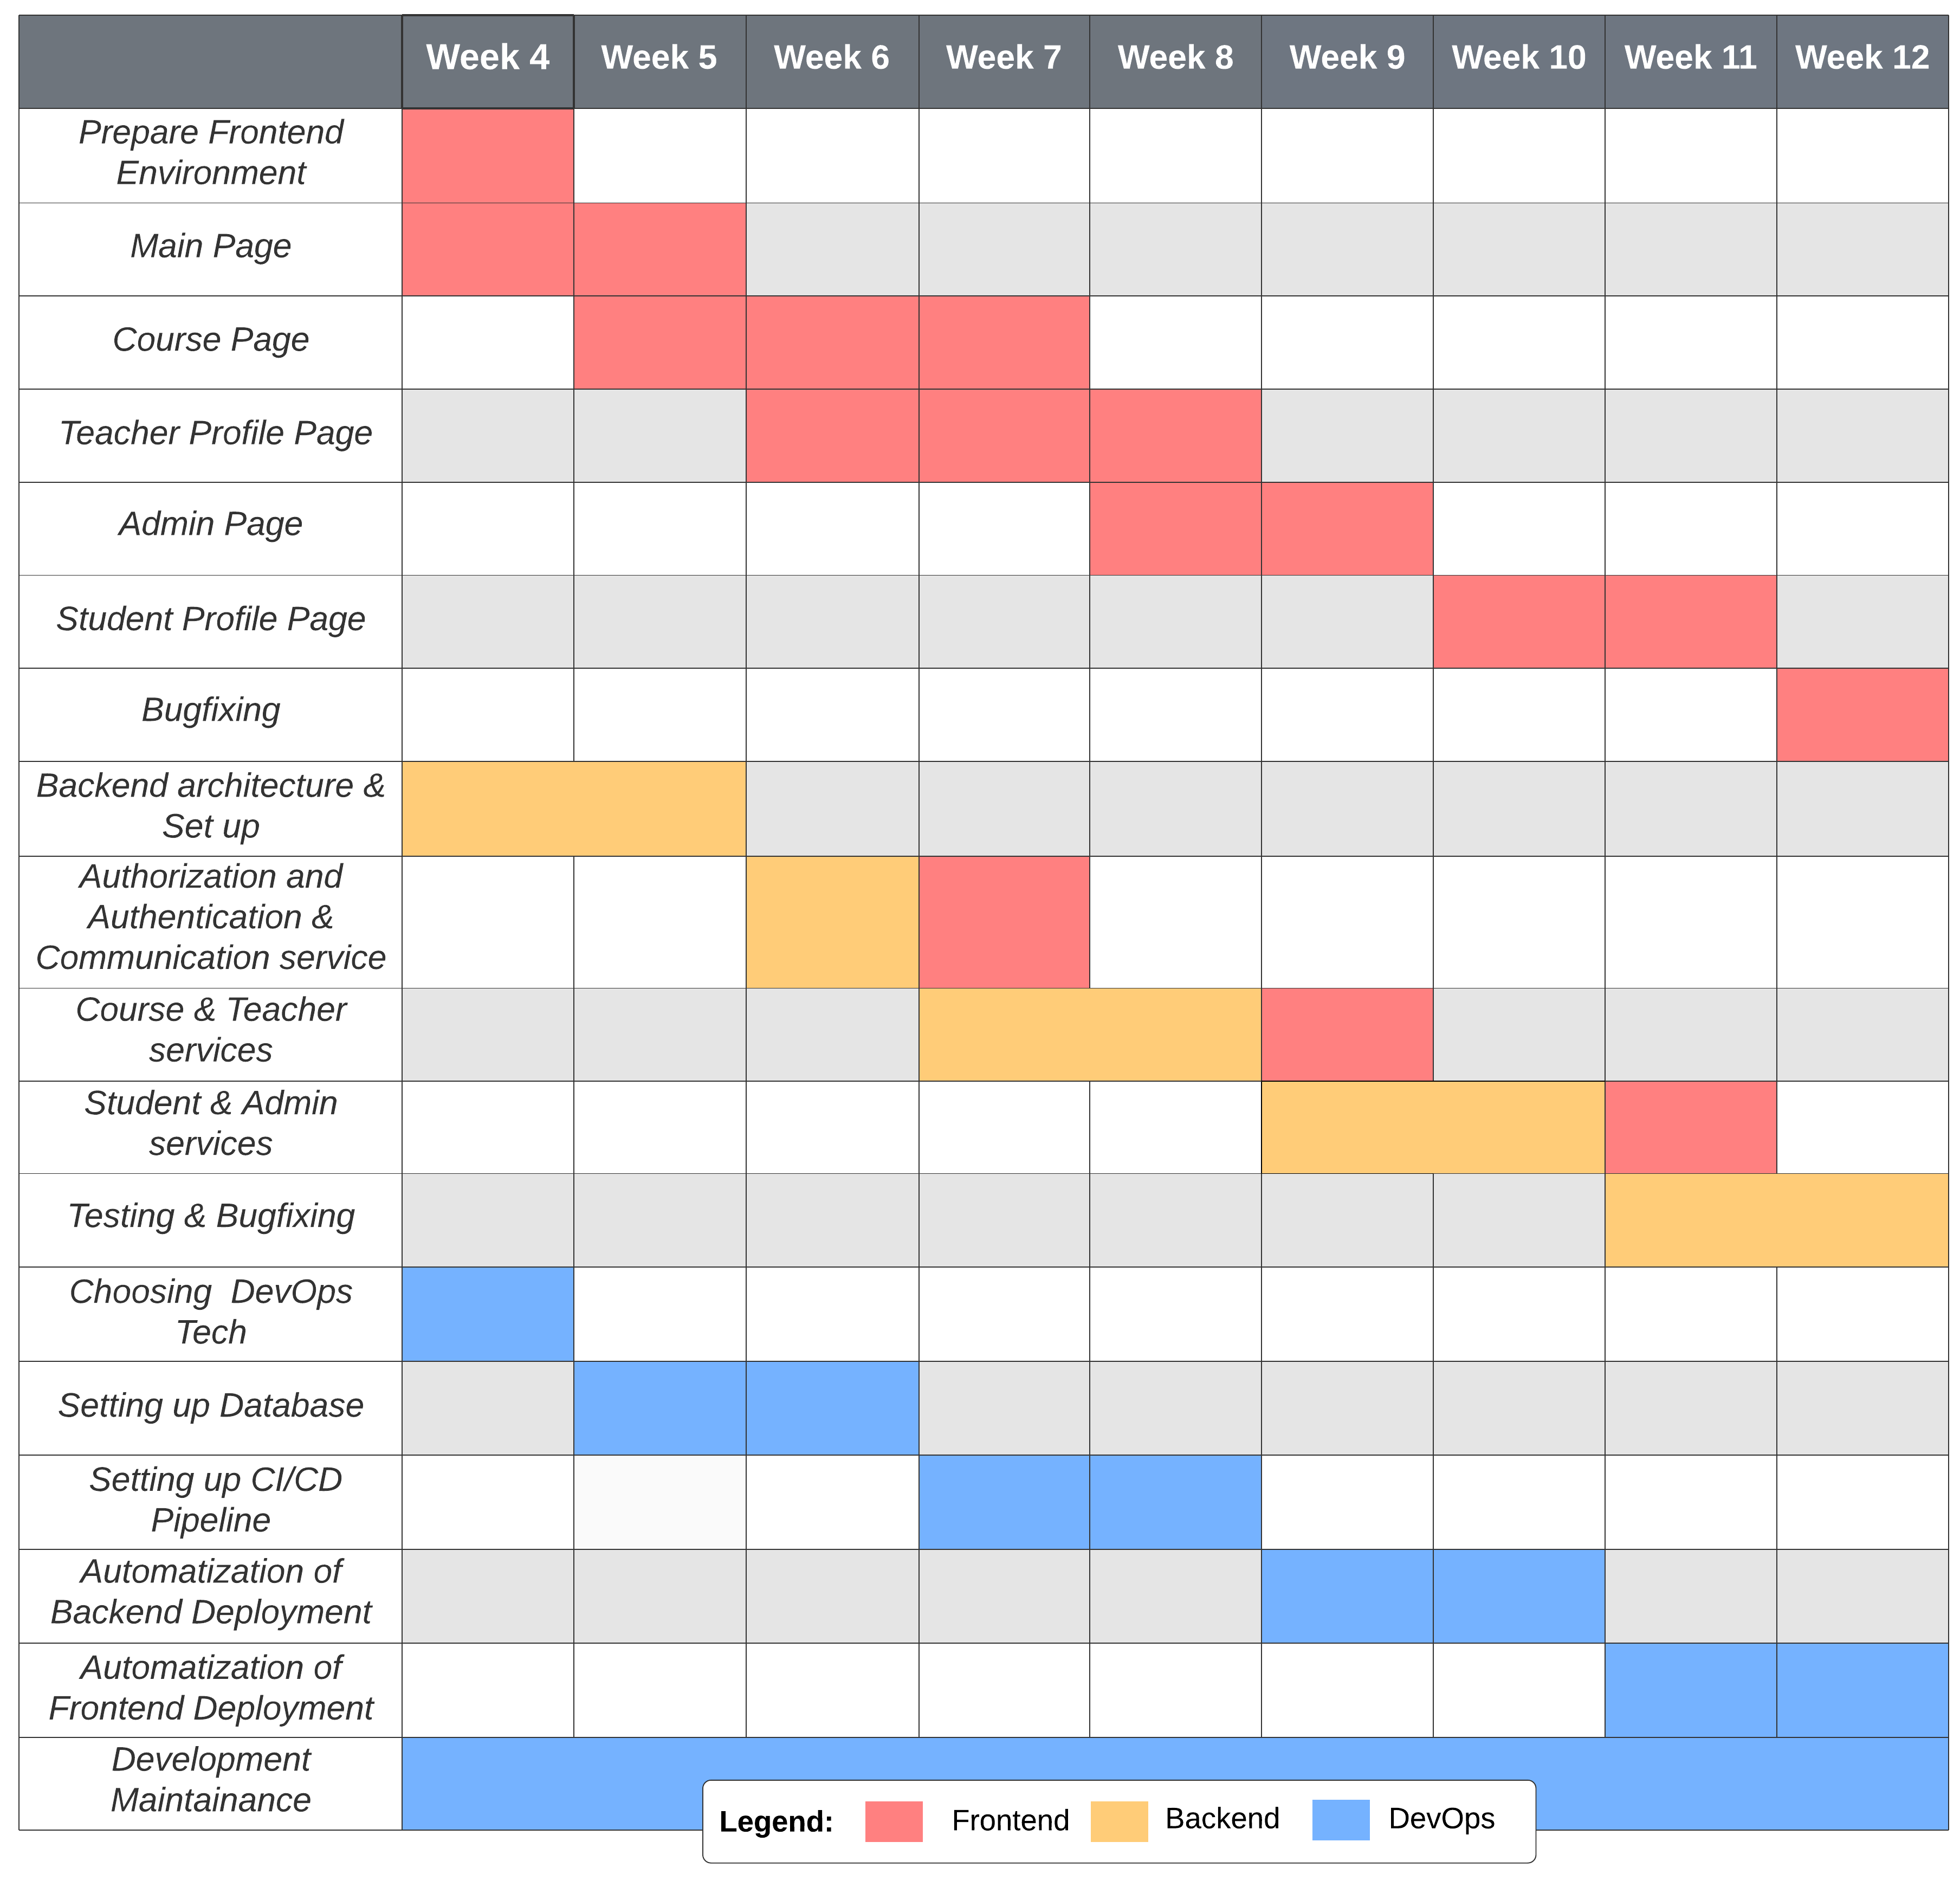
\includegraphics[scale=.52]{img/gantt.png}
    \caption{Gantt chart by task and person}
\end{figure}
\end{center}

\chapter*{Functional Requirements}
\markboth{}{Functional Requirements}
\addcontentsline{toc}{chapter}{Functional Requirements}

We have decided to describe functionality of the platform from the perspective of users, given some specific rights and corresponding access level (roles). This allows us to represent functional requirements of the platform as a set of granular user stories and set of permission levels at the same time.

The roles are as follows:
\begin{itemize}
\itemsep0em 
\addtolength{\itemindent}{0.5cm}
    \vspace{-0.2cm}\item Everyone (combines all the groups below)
    \vspace{-0.2cm}\item Anonymous User (Unauthorised)
	  \vspace{-0.2cm}\item Everyone Authorised (all the groups below)
    \vspace{-0.2cm}\item Teacher
    \vspace{-0.2cm}\item Student
    \vspace{-0.2cm}\item Administrator
\end{itemize}

\begin{enumerate}
	\itemsep0em 
    \item \textbf{Everyone} can: 
    \begin{itemize}
        \vspace{-0.2cm}\item View universities that has been made public
        \vspace{-0.2cm}\item View university courses (and its contents) that has been made public
        \vspace{-0.2cm}\item Search for courses by name, university, tags
    \end{itemize}
    
    \item \textbf{Anonymous User} can :
    \begin{itemize} \itemsep0em 
        \vspace{-0.2cm}\item Login to the existing account
        \vspace{-0.2cm}\item Request the creation of the university account (administrator)
    \end{itemize}
    
    \item \textbf{Authenticated User} can:
     \begin{itemize} \itemsep0em 
      \vspace{-0.2cm}\item Log out
      \vspace{-0.2cm}\item Change personal details
      \vspace{-0.2cm}\item See their University details (if they are hidden from anonymous users)
      \vspace{-0.2cm}\item See their events calendar
      \vspace{-0.2cm}\item Leave messages on university / courses boards
    \end{itemize}

    \item \textbf{Teacher} can :
     \begin{itemize} \itemsep0em 
      \vspace{-0.2cm}\item Change own course information
      \vspace{-0.2cm}\item Appoint events (exams, terms, meetings)
      \vspace{-0.2cm}\item Add materials to the course (videos, text, pdfs, quizes)
    \end{itemize}
    
    \item \textbf{University Administrator} can :
    \begin{itemize} \itemsep0em 
      \vspace{-0.2cm}\item Review submitted university courses
      \vspace{-0.2cm}\item Accept university submitted courses
      \vspace{-0.2cm}\item Reject university submitted courses
      \vspace{-0.2cm}\item Delete university courses (with possibility to recover)
      \vspace{-0.2cm}\item See university students' and teachers' details
      \vspace{-0.2cm}\item Make university courses open
      \vspace{-0.2cm}\item Create teacher / student accounts 
      \vspace{-0.2cm}\item Delete teacheer / student accounts
    \end{itemize}
\end{enumerate}

There is also a super-admin role foreseen, which should be used for resolving software-specific issues and support existing users.

\chapter*{Non-Functional Requirements}
\markboth{}{Non-Functional Requirements}
\addcontentsline{toc}{chapter}{Non-Functional Requirements}

\begin{enumerate}
\itemsep0em 
    \item \textbf{Usability} \\
     Level of basic user expertise assumed. User interface standards will be used.
    \item \textbf{Reliability} \\
      Platform will be available 24/7 with the possibility of restarting the system in case of emergency situations (using PaaS / IaaS functionality or kubernetes). Recoverability will be maintained by an engineer who will recover system from a shut-down failure (in case of several unsuccessful attempts to restart). It will accessible from the most popular browsers like Google Chrome (and Chromium-based), Safari, Firefox, and Opera.

    \item \textbf{Performance} \\
     System response time is supposed to not exceed 2000ms (2 seconds), automatic recovery and start-up time is expected to take up to 30 minutes. 
     
    \item \textbf{Supportability} \\
     System should be testable, maintainable and easily scalable for the needs of higher throughput of media streaming for large number of students. This includes possibility of refactoring the architecture to be more decoupled. 
     
     \item \textbf{Extendibility} \\ 
     System should be easy to extend - meaning it should be possible to add more features to the existing architecture without significant need for the refactoring of previously implemented system. 
     
\end{enumerate}

\chapter*{SWOT Analysis}
\markboth{}{SWOT Analysis}
\addcontentsline{toc}{chapter}{SWOT Analysis}
\begin{tcbraster}[raster columns=2, boxrule=0mm, arc=0mm]
  \singlespacing
\begin{tcolorbox}[equal height group=A, size=fbox, colback=swotS!60, colframe=swotS!80!black, title=\textsc{strengths}]
\begin{enumerate} \itemsep0em 
\item Budget \& support from the university for hosting
\item Previous experience in developing commercial software
\item Strong believe in the right cause and passion for the project
\item Milestones are well-defined and understood
\item Strong support from the Rust and F\# communities
\end{enumerate}
\end{tcolorbox}
\begin{tcolorbox}[equal height group=A, size=fbox, colback=swotW!60, colframe=swotW!80!black, title=\textsc{weaknesses}]
\begin{enumerate} \itemsep0em 
\item Lack of experience with functional paradigm for big projects
\item Lack of expertise in the educatinal domain
\item Lack of experience in the selected technologies
\end{enumerate}
\end{tcolorbox}
\begin{tcolorbox}[equal height group=B, size=fbox, colback=swotO!60, colframe=swotO!80!black, title=\textsc{opportunities}]
\begin{enumerate} \itemsep0em 
\item Growing interest in educational products gives more confidence in the success of the product
\item Modernization of the market of educational websites  
\item Popularization of the functional programming paradigm
\item Building ground for future projects in the sphere 
\end{enumerate}
\end{tcolorbox}
\begin{tcolorbox}[equal height group=B, size=fbox, colback=swotT!60, colframe=swotT!80!black, title=\textsc{threats}]
\begin{enumerate} \itemsep0em 
\item Not enough time to complete the project
\item Absence of team members due to some reasons
\end{enumerate}
\end{tcolorbox}
\end{tcbraster}
\textbf{Threats}
\begin{enumerate}
     \item \textit{Not enough time to complete the project} - there is a possibility that we will not be able to complete all the functional requirements on time. As the project plan itself is quite big, we will simply cut the functionality and leave it for the future - the core goal of experimenting with the technologies in the domain should be achieved in every outcome. 
    \item \textit{Absence of team members due to some reasons} - in this case the left member will evaluate their powers and the amount of work left to do and either ask for permission to continue project alone or end it for the time being. 
\end{enumerate}

\begin{thebibliography}{20} % IF YOU HAVE MORE REFERENCES, WRITE THE BIGGER NUMBER

\bibitem[1]{growth} Dhawal Shah, By The Numbers: MOOCs in 2020, \emph{The Report by class central}, \href{https://www.classcentral.com/report/mooc-stats-2020/}{https://www.classcentral.com/report/mooc-stats-2020/}, Nov 30th, 2020
\bibitem[2]{onvsoff1} A Comparative Study on Effectiveness of Online and Offline Learning in Higher Education, \emph{International Journal of Tourism \& Hospitality in Asia Pasific (IJTHAP) Vol. 4 No. 3, 102-114, October, 2021}  \href{https://www.researchgate.net/publication/355433669_A_Comparative_Study_on_Effectiveness_of_Online_and_Offline_Learning_in_Higher_Education}{https://www.researchgate.net/publication/355433669\_A\_Comparative\_Study\_on\_\\Effectiveness\_of\_Online\_and\_Offline\_Learning\_in\_Higher\_Education}
\bibitem[3]{dropout} "Why Do Students Drop Out of MOOCs?", Rachelle Peterson, National Association of Scholars, \href{https://www.nas.org/blogs/article/why_do_students_drop_out_of_moocs}{https://www.nas.org/blogs/article/why\_do\_students\_drop\_out\_of\_moocs}, November 12, 2013
\bibitem[4]{expectancy} World Life Expectancy 1950-2022, \href{https://www.macrotrends.net/countries/WLD/world/life-expectancy}{https://www.macrotrends.net/countries/WLD/world/life-expectancy}
\bibitem[5]{pace} "Pace of Life and Enjoyment of Life", February 2002, Journal of Happiness Studies 3(3):217-256 \href{https://www.researchgate.net/publication/23545478_Pace_of_Life_and_Enjoyment_of_Life}{https://www.researchgate.net/publication/23545478\_Pace\_of\_Life\_and\_Enjoyment\_of\\\_Life}
\bibitem[6]{harvard1} "Education Now: What Makes a High-Quality Remote or Hybrid Learning Experience?", Harvard Graduate School of Education, \href{https://www.youtube.com/watch?v=EFA9S09ysMc&t=1276s}{https://www.youtube.com/watch?v=EFA9S09ysMc\&t=1276s}
\bibitem[7]{rust} Rust programming language, \href{https://www.rust-lang.org}{https://www.rust-lang.org}
\bibitem[8]{fsharp} F\# programming language, \href{https://fsharp.org}{https://fsharp.org}
\bibitem[9]{fable} Fable compiler (from F\# to JavaScript), \href{https://fable.io}{https://fable.io}
\bibitem[10]{null} Null References: The Billion Dollar Mistake, \href{https://www.infoq.com/presentations/Null-References-The-Billion-Dollar-Mistake-Tony-Hoare/}{https://www.infoq.com/presentations/Null-References-The-Billion-Dollar-Mistake-Tony-Hoare/}
\end{thebibliography}


	
\pagenumbering{gobble}
\thispagestyle{empty}

% ----------------------------  LIST OF FIGURES --------------------------------
\listoffigures
\thispagestyle{empty}

\end{document}
